%%%%%%%%%%%%%%%%%%%%%%%%%%%%%%%%%%%%%%%%%%%%%%%%%%%%%%%%%%%%%%%%%%%%%%%%%%
%% Review Volume (last updated on 2014/03/05) %%
%% Trim Size: 9.61in x 6.69in %%
%% Text Area: 8in (include runningheads) x 5in %%
%% Main Text: 10 on 13pt %%
%% For support: Yolande Koh, <ykoh@wspc.com.sg> %%
%% D. Rajesh Babu, <rajesh@wspc.com.sg> %%
%%%%%%%%%%%%%%%%%%%%%%%%%%%%%%%%%%%%%%%%%%%%%%%%%%%%%%%%%%%%%%%%%%%%%%%%%%
%%
%\documentclass[wsdraft]{ws-rv961x669} % to draw border line around text area
%\documentclass{ws-rv961x669}
\documentclass[addchapnum]{ws-rv961x669} % to add chapter number in volume
\usepackage{ws-rv-van} % numbered citation/references (default)
%\usepackage{ws-rv-thm} % comment this line when `amsthm / theorem / ntheorem` package is used
%\usepackage{subfigure} % required only when side-by-side / subfigures are used
\usepackage{ws-index} % required only when multiple indexes are used
%\usepackage[colorlinks=false]{hyperref}
%\usepackage{doi}
\usepackage{bbm}
\usepackage{amsmath}
\usepackage{amssymb}
\makeindex
\newindex{aindx}{adx}{and}{Author Index} % author index
\renewindex{default}{idx}{ind}{Subject Index} % subject index

\newcommand{\req}[1]{Eq.~(\ref{#1})}
\newcommand{\rsec}[1]{Sec.~{\ref{#1}}}

\begin{document}

\chapter[Dynamic flavor mixing through transition moments]{Dynamic flavor mixing through transition moments\label{JR_ch1}}

\author[J. Rafelski and A. Steinmetz]{Johann Rafelski and Andrew Steinmetz\footnote{JohannR@Arizona.EDU, AJSteinmetz@Arizona.EDU}}
\aindx{Rafelski, J.}
\aindx{Steinmetz, A.}

\address{Department of Physics, The University of Arizona, Tucson, AZ 85721, USA}

\begin{abstract} 
As neutrinos are naturally massless in the standard model the observed flavor oscillation presents a mystery. Moreover it is unknown if neutrinos are Dirac-type or Majorana-type fermions. We show that Majorana neutrino flavor mixing can be driven by electromagnetic transition dipole moments. We analyze neutrino eigenstates in a two-flavor model and the sensitivity of the rotation mixing matrix to strong electromagnetic fields. Matter interactions and the three-flavor oscillations are discussed. We postulate mass generation via neutrino dipole coupling to a dark vector field.
\end{abstract}

\markboth{Johann Rafelski and Andrew Steinmetz}{Neutrinos in EM fields} % Customized running heads

\body

%\tableofcontents\

%%%%%%%%%%%%%%%%%%%%%%%%%%%%%%%%%%%%
\section{Introduction}
\label{sec:intro}
%%%%%%%%%%%%%%%%%%%%%%%%%%%%%%%%%%%%

In this work we look at the connection between neutrino transition magnetic dipole moments~\cite{Fujikawa:1980yx,Shrock:1980vy,Shrock:1982sc} and neutrino flavor oscillation. Neutrinos once were the dominant form of energy density in the universe~\cite{Rafelski:2023emw} and are also important in the context of stellar evolution and supernova. There is profound interest in understanding their physical properties due to their importance as a bridge to beyond standard model (BSM) physics~\cite{DUNE:2020fgq}. It is also unknown which (normal or inverted) hierarchy neutrinos follow therefore probing the EM properties of neutrinos could contribute evidence for one model over the other~\cite{Kouzakov:2023jtt}. Their electromagnetic (EM) properties have been considered before~\cite{Schechter:1981hw,Giunti:2014ixa,Chukhnova:2019oum,Popov:2019nkr} but to best of our knowledge this is a first consideration of the full EM contribution to flavor oscillation.

As neutrinos are electrically neutral, they have no intrinsic magnetic moment due to their spin, therefore any nonzero dipole moment is considered anomalous~\cite{Steinmetz:2018ryf}. A small anomalous magnetic moment (AMM) can be introduced into the neutrino Lagrangian via a Pauli term. Transition magnetic moments are moments which couple different flavor electromagnetically. Since transition AMM elements serve to break lepton number conservation allowing for $\nu_{\ell}+\gamma\rightarrow\nu_{\ell'}$ processes where $\ell$ and $\ell\,'$ are different lepton flavors, neutrinos could be remixed when exposed to strong EM fields similar to remixing within matter in the Mikheyev-Smirnov-Wolfenstein (MSW) effect~\citep{Wolfenstein:1977ue,Mikheyev:1985zog}.

The size of the neutrino magnetic dipole moment is relatively small with a lower bound determined by the standard model~\cite{Fujikawa:1980yx,Shrock:1980vy,Shrock:1982sc} and an upper bound from (reactor and solar) experimental observations~\cite{Giunti:2015gga,Canas:2015yoa,Studenikin:2016ykv,AristizabalSierra:2021fuc} given by
\begin{align}
    \label{bound:1}
    \frac{e\hbar G_{F}m_{\nu}c^{2}}{8\pi^{2}\sqrt{2}} \sim 10^{-19}\mu_{B}<\mu_{\nu}^\mathrm{eff}<10^{-10}\mu_{B}\,,\qquad\mu_{B}=\frac{e\hbar}{2m_{e}}
\end{align}
where $\mu_{B}$ is the Bohr magneton and $\mu_{\nu}^\mathrm{eff}$ is the effective and characteristic size of the neutrino magnetic moment. In \req{bound:1} $G_{F}$ is the Fermi constant and $m_{\nu}$ the neutrino mass.

Considering higher order standard model diagrams neutrino should manifestation non-minimal EM interactions~\citep{Giunti:2014ixa} of the form
\begin{align}
    \label{mu:1}
    \mu_{\ell\ell'}=
	\begin{pmatrix}
		\mu_{ee} & \mu_{e\mu} & \mu_{e\tau} \\
		\mu_{\mu e} & \mu_{\mu\mu} & \mu_{\mu\tau} \\
		\mu_{\tau e} & \mu_{\tau\mu} & \mu_{\tau\tau}
	\end{pmatrix}\,,
\end{align}
where $\ell$ are the neutral lepton flavor indices $\ell\in\nu_{e},\nu_{\mu},\nu_{\tau}$. The transition moments are considered smaller than direct moments, but BSM physics or non-standard neutrinos~\cite{Giunti:2014ixa} are capable of producing an abnormally large electromagnetic dipole~\citep{Ohlsson:2012kf,Lindner:2017uvt,Brdar:2020quo} within the bounds of~\req{bound:1} which may manifest itself in strong field or/and dense matter environments.

%%%%%%%%%%%%%%%%%%%%%%%%%%%%%%%%%%%%%%%
\section{Neutrino flavor mixing and electromagnetic fields}
\label{sec:nuflavor}
%%%%%%%%%%%%%%%%%%%%%%%%%%%%%
Experiment shows that neutrino mass and flavor eigenstates differ. This misalignment between the two representations is described as rotation of the neutrino flavor $N$-vector where $N=3$ is the observed number of generations. The unitary mixing matrix $V_{\ell k}$ allows for the change of basis between mass $(k)$ and flavor $(\ell)$ eigenstates via the transform 
\begin{alignat}{1}
	\label{basis:1} \nu_{\ell}=\sum_{k=1}^{3}V_{\ell k}\nu_{k}\,\rightarrow
	\begin{pmatrix}
		\nu_{e}\\
		\nu_{\mu}\\
		\nu_{\tau}
	\end{pmatrix}=
	\begin{pmatrix}
		V_{e1} & V_{e2} & V_{e3}\\
		V_{\mu1} & V_{\mu2} & V_{\mu3}\\
		V_{\tau1} & V_{\tau2} & V_{\tau3}
	\end{pmatrix}
	\begin{pmatrix}
		\nu_{1}\\
		\nu_{2}\\
		\nu_{3}
	\end{pmatrix}\,,
\end{alignat}
where $\nu_{\ell}$ is the neutrino state four-spinor written in the flavor basis while in the mass basis we use $\nu_{k}$ with $k\in1,2,3$. Hereafter we will use implied summation  over repeated flavor indices. Spinor indices will be suppressed.

The parameterization of the components of the mixing matrix depends on the Dirac or Majorana-nature of the neutrinos. We consider $U_{\ell k}$ to be the Dirac neutrino mixing matrix which in the standard parameterization~\citep{Schwartz:2014sze}, can be expressed as
\begin{alignat}{1}
	\label{rotation:1} U_{\ell k} =
	  \begin{pmatrix}
		  c_{12}c_{13} & s_{12}c_{13} & s_{13}e^{-i\delta}\\
		  -s_{12}c_{23} - c_{12}s_{13}s_{23}e^{i\delta} & c_{12}c_{23} - s_{12}s_{13}s_{23}e^{i\delta} & c_{13}s_{23}\\
		  s_{12}s_{23} - c_{12}s_{13}c_{23}e^{i\delta}& -c_{12}s_{23} - s_{12}s_{13}c_{23}e^{i\delta} & c_{13}c_{23}
	  \end{pmatrix}\,,
\end{alignat}
where $c_{ij} = \mathrm{cos}(\theta_{ij})$ and $s_{ij} = \mathrm{sin}(\theta_{ij})$. In this convention, the three mixing angles $(\theta_{12}, \theta_{13}, \theta_{23})$, are understood to be the Euler angles for generalized rotations and $\delta$ is the CP-violating complex phase. 

For the Majorana case of interest to us we must allow a greater number of complex phases described by an additional phase matrix $P_{kk'}$
\begin{alignat}{1}
	\label{phases:1} &V_{\ell k} = U_{\ell k'}P_{k'k}\,,\\
	\label{phases:3} &P_{kk'} = \mathrm{diag}(e^{i\rho},e^{i\sigma},1)\,.
\end{alignat}
Majorana neutrinos allow up to two additional complex phases $\rho$ and $\sigma$ which along with $\delta$ participate in CP-violation. The mixing matrix $V_{\ell k}$ defined in \req{phases:1} can then be used to diagonalize the mass matrix $M$ from the flavor basis into the mass basis as
\begin{align}
    \label{diag:1}
    V_{\ell k}^{T}M_{\ell\ell'}V_{\ell'k'} = M_{kk'} = m_{k}\delta_{kk'} = \mathrm{diag}(m_{1},m_{2},m_{3})\,.
\end{align}
The masses $m_{k}$ are taken to be real and positive labelling the free propagating states of the three neutrinos.

Turning now to the action, 
the Majorana mass term in the Lagrangian can be written in the Weyl (chiral) flavor basis as
\begin{alignat}{1}
	\label{mass:1} \mathcal{L}_{\mathrm{mass}}^{\mathrm{Maj.}}=\frac{1}{2}\nu_{L,\ell}^{T}C^{\dag}M_{\ell\ell'}\nu_{L,\ell'}+\mathrm{h.c}\,,\qquad
    M_{\ell\ell'}^{T}=M_{\ell\ell'}\,,
\end{alignat}
where $\nu_{L}$ refers to left-handed chiral four-component spinors. We do not consider right-handed neutrino states. We note the Majorana mass matrix is symmetric due to the anticommuting nature of the neutrino fields and is in general complex~\cite{Adhikary:2013bma}. The charge conjugation matrix $C$ is defined in Ref.~\citeauthor{Itzykson:1980rh}, p.692.

Given these conventions, we can extend our consideration to include interactions of neutrinos with an \underline{externally given} electromagnetic field tensor $F^{\alpha\beta}$ with an externally prescribed field $A^{\alpha}_\mathrm{ext}(x)$ which imparts a force on the neutrino fields. This is possible if neutrinos are equipped with a magnetic moment matrix $\mu_{\ell\ell'}$. 

We generalize the usual Pauli spin-field AMM coupling Lagrangian to account for the Majorana fields in the flavor basis following the approach of Ref.~\citeauthor{giunti2007fundamentals}
\begin{align}
	\label{moment:1}
    \mathcal{L}_{\mathrm{AMM}}^\mathrm{Maj.}=\frac{1}{2}\nu_{L,\ell}^{T}C^{\dag}\left(\mu_{\ell\ell'}\frac{1}{2}\sigma_{\alpha\beta}F^{\alpha\beta}\right)\nu_{L,\ell'}+\mathrm{h.c.}
\end{align}
The operator $\sigma_{\alpha\beta}$ is the $4\times 4$ spin tensor defined by the commutator of the gamma matrices. We would like to point out some interesting features of the Pauli term most notably that the spin tensor itself is not Hermitian with
\begin{align}
    \label{notherm:1}
    \sigma_{\alpha\beta}^{\dag} = \gamma_{0}\sigma_{\alpha\beta}\gamma_{0}
\end{align}
Despite this, the Lagrangian term in \req{moment:1} is still itself Hermitian. This is easier to see when the fields are written as Majorana spinors $\nu=\nu_{L}+C\gamma_{0}\nu_{L}^{*}$
\begin{align}
    \left(\nu^{\dag}\gamma_{0}\sigma_{\alpha\beta}F^{\alpha\beta}\nu\right)^{\dag} = \nu^{\dag}\sigma_{\alpha\beta}^{\dag}F^{\alpha\beta}\gamma_{0}\nu = \nu^{\dag}\gamma_{0}\sigma_{\alpha\beta}F^{\alpha\beta}\nu\,,
\end{align}
which is Hermitian as promised. More about the spin tensor's properties will be elaborated on in \rsec{sec:numoment}.

The magnetic moment matrix acts in flavor space (see \req{mu:1}) and it satisfies for CPT reasons the following constraints~\cite{Giunti:2014ixa}
\begin{alignat}{1}
	\label{props:1}
    \mu_{\ell\ell'}^{\dag}=\mu_{\ell\ell'}\,,\qquad
    \mu_{\ell\ell'}^{T}=-\mu_{\ell\ell'}\,,
\end{alignat}
{\it i.e.\/} the AMM matrix $\mu_{\ell\ell'}$ is Hermitian and fully anti-symmetric. This requires that the transitional magnetic moment elements are purely imaginary while all diagonal AMM matrix elements vanish
\begin{align}
    \mu_{\ell\ell'}=
    \begin{pmatrix}
        0 & i\mu_{e\mu} & -i\mu_{e\tau} \\
		-i\mu_{e\mu} & 0 & i\mu_{\mu\tau} \\
		i\mu_{e\tau} & -i\mu_{\mu\tau} & 0
    \end{pmatrix}\,.
\end{align}

We can combine the AMM contribution and the mass term in~\req{mass:1} and~\req{moment:1} to write an effective Lagrangian containing both
\begin{align}
	\label{massmom:1}
    \mathcal{L}_\mathrm{eff}^\mathrm{Maj.} =
    \mathcal{L}_\mathrm{mass}^\mathrm{Maj.} + \mathcal{L}_\mathrm{AMM}^\mathrm{Maj.} = 
    \frac{1}{2}\nu_{L,\ell}^{T}C^{\dag}\left(M_{\ell\ell'}+\mu_{\ell\ell'}\frac{1}{2}\sigma_{\alpha\beta}F^{\alpha\beta}\right)\nu_{L,\ell'}+\mathrm{h.c.}
\end{align}
\req{massmom:1} will be our working Lagrangian for the majority of our work. We define the generalized mass-dipole matrix $\mathcal{M}_{\ell\ell'}$ present in \req{massmom:1} as
\begin{align}
	\label{massmom:2}
    \mathcal{M}_{\ell\ell'}(E,B)\equiv M_{\ell\ell'}+\mu_{\ell\ell'}\frac{1}{2}\sigma_{\alpha\beta}F^{\alpha\beta}\,.
\end{align}
As neutrinos must propagate as energy eigenstates, our objective is to find the eigenvalues of \req{massmom:2} rather than \req{diag:1}. As the mass eigenvalues are modified by the presence the EM interactions $m\rightarrow\widetilde m(E,B)$ so will the mixing matrix, leading to modifications to \req{phases:1}. These electromagnetic components then facilitate time-dependant oscillation among the free-particle mass eigenstates~\cite{Giunti:2014ixa}.

Additionally, we may consider matter effects via the weak interaction. Electron (anti)neutrinos passing through matter preferentially interact via weak charge current (CC) with electrons which make up the bulk of charged leptons in most matter. The neutral current (NC) however affects all flavors and couples to the neutrons within the medium (as the electron and proton contributions cancel in charge neutral matter). This can be represented as the potentials~\cite{Pal:1991pm,greiner2009gauge} $V_{CC}$ and $V_{NC}$ which contribute to the action as
\begin{align}
    \label{matter:1}
    \mathcal{L}_\mathrm{matter}^\mathrm{Maj.} &= \nu_{L,\ell}^{\dag}\gamma_{0}V_{\ell\ell'}\gamma_{0}\nu_{L,\ell'}\,,\qquad
    V_{\ell\ell'} = 
    \begin{pmatrix}
        V_{CC}+V_{NC} & 0 & 0\\
        0 & V_{NC} & 0\\
        0 & 0 & V_{NC}
    \end{pmatrix}\,,\\
    V_{CC} &= \sqrt{2}G_{F}\hbar^{2}c^{2}n_{e}\,,\qquad V_{NC} = -\frac{1}{2}\sqrt{2}G_{F}\hbar^{2}c^{2}n_{n}\,.
\end{align}
The coefficient $G_{F}$ is the Fermi constant, $n_{e}$ is the number density of electron matter and $n_{n}$ is the number density of neutrons within the medium. We note that $V_{\ell\ell'}\gamma_{0}$ behaves like the zeroth component of a vector-potential.

%%%%%%%%%%%%%%%%%%%%%%%%%%%%%%%%%%%%%%%
\section{Properties of Pauli coupling to EM fields}
\label{sec:numoment}
%%%%%%%%%%%%%%%%%%%%%%%%%%%%%%%%%%%%%%%
The electromagnetic dipole behavior of the neutrino depend on mathematical properties of the tensor product $\sigma_{\alpha\beta}F^{\alpha\beta}$. We prefer to work in the Weyl (chiral) spinor representation where the EM contribution is diagonal in spin space. Therefore we evaluate the product $\sigma_{\alpha\beta}F^{\alpha\beta}$ in the chiral representation following Feynman and Gell-mann\cite{Feynman:1958ty} yielding
\begin{align}
    \label{chiral:1}
    -\frac{1}{2}\sigma_{\alpha\beta}F^{\alpha\beta}=
    \begin{pmatrix}
        \vec{\sigma}\cdot(\vec{B}+i\vec{E}/c) & 0\\
        0 & \vec{\sigma}\cdot(\vec{B}-i\vec{E}/c)
    \end{pmatrix}\equiv
    \begin{pmatrix}
        \vec{\sigma}\cdot\vec{f}_{+} & 0 \\
        0 & \vec{\sigma}\cdot\vec{f}_{-}
    \end{pmatrix}\,,
\end{align}
where we have defined the complex electromagnetic field $\vec{f}_{\pm}=\vec{B}\pm i\vec{E}/c$. As \req{chiral:1} is diagonal in this representation, it does not exchange handedness when acting upon a state. This expression also shows directly that neutrinos are not only sensitive to magnetic, but electric fields as well which is often neglected in theoretical neutrino studies.

We can also see in \req{chiral:1} the explicitly non-Hermitian character of the complex EM fields $\vec{f}_{\pm}$ as $(\vec{f}_{\pm})^{*}=\vec{f}_{\mp}$. More specifically, the complex EM fields have a Hermitian $(\vec{B})$ and anti-Hermitian $(i\vec{E})$ part.

For later convenience we note how the EM invariants $\mathcal{S}$ and $\mathcal{P}$ can help understand the AMM term 
\begin{align}
    \label{invar:1}
    \left(\frac{1}{2}\sigma_{\alpha\beta}F^{\alpha\beta}\right)^{2}=
    \begin{pmatrix}
        \mathcal{S}+i\mathcal{P} & 0\\
        0 & \mathcal{S}-i\mathcal{P}
    \end{pmatrix}=\mathcal{S}-i\gamma_{5}\mathcal{P}\,,\\
    \mathcal{S}\equiv\frac{1}{2}\left(B^{2}-E^{2}/c^{2}\right)\,,\qquad
    \mathcal{P}\equiv\vec{B}\cdot\vec{E}/c\,,\qquad
    \frac{1}{2}\vec{f}_{\pm}\cdot\vec{f}_{\pm}=\mathcal{S}\pm i\mathcal{P}\,.
\end{align}
The combination of these invariants make up the eigenvalues of the Pauli term. Moreover, for the product of $\vec{f}_{\pm}$ with its complex conjugate we find
\begin{align}
        \label{cross:1}
        \frac{1}{2}\left(\vec{\sigma}\cdot\vec{f}_{\pm}\right)\left(\vec{\sigma}\cdot\vec{f}_{\mp}\right)=T^{00}\mp \sigma_{i}T^{0i}\,,
\end{align}
where we recognize the stress-energy tensor $T^{\alpha\beta}$ component $T^{00}$ for field energy density and $T^{0i}$ momentum density respectively
\begin{align}
    T^{00}=\frac{1}{2}\left(B^{2}+E^{2}/c^{2}\right)\,,\qquad
    T^{0i}=\frac{1}{c}\varepsilon_{ijk}E_{j}B_{k}\,.
\end{align}
As we will see in \rsec{sec:toy}, \req{cross:1} will appear in the mass eigenvalues of our effective Lagrangian \req{massmom:1}. Using the identity in \req{chiral:1} and \req{cross:1} we also find the interesting relationship
\begin{align}
    \label{cross:2}
    \frac{1}{2}\left(\sigma_{\alpha\beta}F^{\alpha\beta}\right)\left(\sigma_{\alpha\beta}F^{\alpha\beta}\right)^{\dag}=
    -\gamma_{\alpha}\left(C^{\dag}\gamma_{\beta}C\right)T^{\alpha\beta}\,.
\end{align}
Now that we have elaborated on the relevant EM field identities, we turn back to the magnetic dipole and flavor oscillation.

%%%%%%%%%%%%%%%%%%%%%%%%%%%%%%%%%%%%%%%
\section{Toy model: Magnetic-flavor mixing for two generations with real Hermitian mass matrix}
\label{sec:toy}
%%%%%%%%%%%%%%%%%%%%%%%%%%%%%%%%%%%%%%%
Considering experimental data on neutrino oscillations, it is understood that either the two heavier (normal hierarchy) or the two lighter (inverted hierarchy) neutrino states are close together in mass. If the electromagnetic properties of the neutrino do indeed lead to flavor mixing effects, then it is likely the closer pair of neutrino mass states that are most sensitive to effective potentials phenomenon. In the spirit of Bethe~\cite{Bethe:1986ej}, we therefore explore the $N=2$ two generation $(\nu_{e},\nu_{\mu})$ model.

Following the properties established in \req{props:1} and \req{massmom:2} we write down the two generation mass and dipole matrices as
\begin{alignat}{1}
	\label{mix:1} M_{\ell\ell'}= 
	\begin{pmatrix}
		m_{\nu_{e}} & {\delta m}\\
		{\delta m} & m_{\nu_{\mu}}
	\end{pmatrix}\,,\qquad
	\mu_{\ell\ell'} = 
	\begin{pmatrix}
		0 & i\delta\mu\\
		-i\delta\mu & 0
	\end{pmatrix}\,.
\end{alignat}
The AMM coupling $\delta\mu$ is taken to be real with a pure imaginary coefficient. While the mass elements $m_{\nu_{e}}$, $m_{\nu_{\mu}}$, and ${\delta m}$ are generally complex, we choose in our toy model for them to be fully real
\begin{align}
    \label{choice:1}
    m_{\nu_{e}}=m_{\nu_{e}}^{*}\,,\qquad
    m_{\nu_{\mu}}=m_{\nu_{\mu}}^{*}\,,\qquad
    \delta m^{*}=\delta m\,,
\end{align}
making the mass matrix $M_{\ell\ell'}$ Hermitian. This allows us to more easily evaluate and emphasize the EM contributions to mixing rather than complications arising from the mass matrix.

Using \req{mix:1} and \req{choice:1}, we write the mass-dipole matrix in \req{massmom:2} in terms of spin-flavor components as
\begin{align}
	\label{mix:2}
    \mathcal{M}_{\ell\ell'} = 
	\begin{pmatrix}
		m_{\nu_{e}} & {\delta m}+i\delta\mu\sigma_{\alpha\beta}F^{\alpha\beta}/2\\
		{\delta m}-i\delta\mu\sigma_{\alpha\beta}F^{\alpha\beta}/2 & m_{\nu_{\mu}}
	\end{pmatrix}\,.
\end{align}
This matrix is however not Hermitian due to the inclusion of the spin tensor as seen in \req{notherm:1}, therefore it is not guaranteed to have real eigenvalues in its present form~\cite{arfken2011mathematical} which is a requirement for well behaved masses.

We note however that the related matrix $\mathcal{M}_{\ell\ell'}\gamma_{0}$ is Hermitian
\begin{align}
    \label{herm:1}
    (\mathcal{M}_{\ell\ell'}\gamma_{0})^{\dag} = \mathcal{M}_{\ell\ell'}\gamma_{0}\,,
\end{align}
and also equivalent to the root of the Hermitian product of \req{mix:2}
\begin{align}
    (\mathcal{M}\mathcal{M}^{\dag})_{\ell\ell'} = \left((\mathcal{M}\gamma_{0})(\mathcal{M}\gamma_{0})\right)_{\ell\ell'}\,.
\end{align}
Therefore for a suitable unitary transformation $W_{\ell j}$ which rotates flavor states into magnetized mass states $(j)$, the eigenvalues $\lambda_{j}^{2}$ of $(\mathcal{M}\mathcal{M}^{\dag})_{\ell\ell'}$ are the squares of the eigenvalues of $\mathcal{M}_{\ell\ell'}\gamma_{0}$ via (with flavor indices suppressed)
\begin{align}
    W^{\dag}(\mathcal{M}_{\ell\ell'}\gamma_{0})W &= \mathrm{diag}(\lambda_{1},\lambda_{2})\,,\\
    W^{\dag}(\mathcal{M}\mathcal{M}^{\dag})W &= W^{\dag}(\mathcal{M}\gamma_{0})WW^{\dag}(\mathcal{M}\gamma_{0})W = \mathrm{diag}(\lambda_{1}^{2},\lambda_{2}^{2})\,.
\end{align}
We associate $\lambda_{j}=\widetilde m_{j}(E,B)$ with the effective magnetized masses which are field dependant in this basis and mix flavor states distinctly from the free-particle case.

Instead of computing $W_{\ell j}$ immediately, it is valuable to break the rotation into two separate unitary transformations that relate flavor to the free mass $(\ell\rightarrow k)$ rotation $V_{\ell k}$ to free mass to the magnetized mass $(k\rightarrow j)$ rotation $Z_{kj}$. Using \req{basis:1}, we write this symbolically as
\begin{align}
    \nu_{j}=Z_{kj}^{\dag}V_{\ell k}^{\dag}\nu_{\ell} = W^{\dag}_{\ell j}\nu_{\ell}\,.
\end{align}
In the limit that $\vec{E}$ and $\vec{B}$ go to zero, the magnetized rotation becomes unity $Z_{kj}\rightarrow\delta_{kj}$ thereby ensuring the magnetized mass basis and free mass basis become equivalent.

According to \req{diag:1}, the mass matrix in \req{mix:1} can be diagonalized in the two generation case by a one parameter unitary mixing matrix $V_{\ell k}$ given by
\begin{align}
    \label{rot:1}
    V_{\ell k}=
    \begin{pmatrix}
        \cos\theta & \sin\theta\\
        -\sin\theta & \cos\theta
    \end{pmatrix}\,.
\end{align}
For a real Hermitian $2\times 2$ mass matrix, the rotation matrix $V_{\ell k}$ only depends on the angle $\theta$. We note for the special case of transition magnetic moment moments, $\mu_{\ell\ell'}$ commutes with the mixing matrix $V_{\ell k}$ and the following relations hold
\begin{align}
    V_{\ell k}^{\dag}\mu_{\ell\ell'}V_{\ell' k'}=(V^{\dag}V)_{k\ell'}\mu_{\ell'k'}=\mu_{kk'}=
    \begin{pmatrix}
        0 & i\delta\mu\\
        -i\delta\mu & 0
    \end{pmatrix}\,.
\end{align}
Therefore applying the free particle rotation $V_{\ell k}$ will simplify the overall mass-dipole matrix in \req{mix:2}. We apply the rotation in \req{rot:1} to \req{herm:1} yielding
\begin{align}
    \label{herm:2}
    V_{\ell k}^{\dag}(\mathcal{M}_{\ell\ell'}\gamma_{0})V_{\ell' k'} &= 
    V_{\ell k}^{\dag}M_{\ell\ell'}\gamma_{0}V_{\ell' k'} +
    V_{\ell k}^{\dag}(\mu_{\ell\ell'}\frac{1}{2}\sigma_{\alpha\beta}\gamma_{0}F^{\alpha\beta})V_{\ell' k'}\,,\\
    \label{herm:3}
    V_{\ell k}^{\dag}(\mathcal{M}_{\ell\ell'}\gamma_{0})V_{\ell' k'} &= 
	\begin{pmatrix}
        m_{1}\gamma_{0} & i\delta\mu\sigma_{\alpha\beta}\gamma_{0}F^{\alpha\beta}/2\\
        -i\delta\mu\sigma_{\alpha\beta}\gamma_{0}F^{\alpha\beta}/2 & m_{2}\gamma_{0}
	\end{pmatrix}\equiv
    \begin{pmatrix}
        A & iC\\
        -iC & B
    \end{pmatrix}\,,
\end{align}
where we've defined the Hermitian elements $(A,B,C)$.

The magnetized mass eigenstates are then solutions to the characteristic polynomial obtained by taking the determinant of \req{herm:3} over flavor but not spin space
\begin{align}
    \label{poly:1}
    (A-\lambda_{j}\gamma_{0})(B-\lambda_{j}\gamma_{0})-C^{2}=0\,,\\
    C^{2} = -\delta\mu^{2}\frac{1}{2}\gamma_{\alpha}(C^{\dag}\gamma_{\beta}C)T^{\alpha\beta} = 
    \delta\mu^{2}\frac{1}{2}\left(T^{00}+\gamma_{5}\sigma_{i}T^{0i}\right)\,,\\
    (A-B)^{2} = \Delta m^{2}\,,\qquad (A+B)\gamma_{0} = m_{1} + m_{2}\,.
\end{align}
Because of the spinor behavior of each element, the eigenvalues are obtained with $\gamma_{0}$ coefficients. \req{poly:1} therefore has the roots
\begin{align}
    \label{poly:2}
    \lambda_{\pm} = \widetilde m_{\pm}(E,B) &= \frac{1}{2}\left((A+B)\gamma_{0}\pm\sqrt{(A-B)^{2}+4C^{2}}\right)\,,\\
    \widetilde m_{\pm}(E,B) &= \frac{1}{2}\left(m_{1}+m_{2}\pm\sqrt{\Delta m^{2}+2\delta\mu^{2}\left(T^{00}+\gamma_{5}\sigma_{i}T^{0i}\right)}\right) 
\end{align}

%%%%%%%%%%%%%%%%%%%%%%%%%%%%%%%%%%%%
\section{Conclusions}
In this work we have described the formalism of including an anomalous dipole moment into the mixing matrix for three generations of Majorana neutrinos and explicitly explored the two generation Majorana neutrino case and determined the effect of magnetic fields on flavor rotation. This signifies a connection between spin and flavor which has not received attention in literature and should be explored for circumstances where strong field electromagnetic fields are present.

An additional consideration of our work is the presence of a dark vector field in the universe which if coupled to neutrinos would behave like off-diagonal masses for nonzero transition magnetic dipoles.

%%%%%%%%%%%%%%%%%%%%%%%%%%%%%%%%%%%%
\section*{Acknowledgements}
Harald Fritzsch enjoyed the US-South-West. On the way between Caltech and the Santa Fe Institute he sometimes made a stop at the half-way point, Tucson. On such occasions he explored Arizona mountains and  deserts; Figure\,\ref{Fig:AZcolloq2007} is showing our outing on occasion of March 23, 2007 physics colloquium at the University of Arizona: Harald was an avid observer and photographer of the desert fauna and flora. 
 
\begin{figure}%[hb]
\centerline{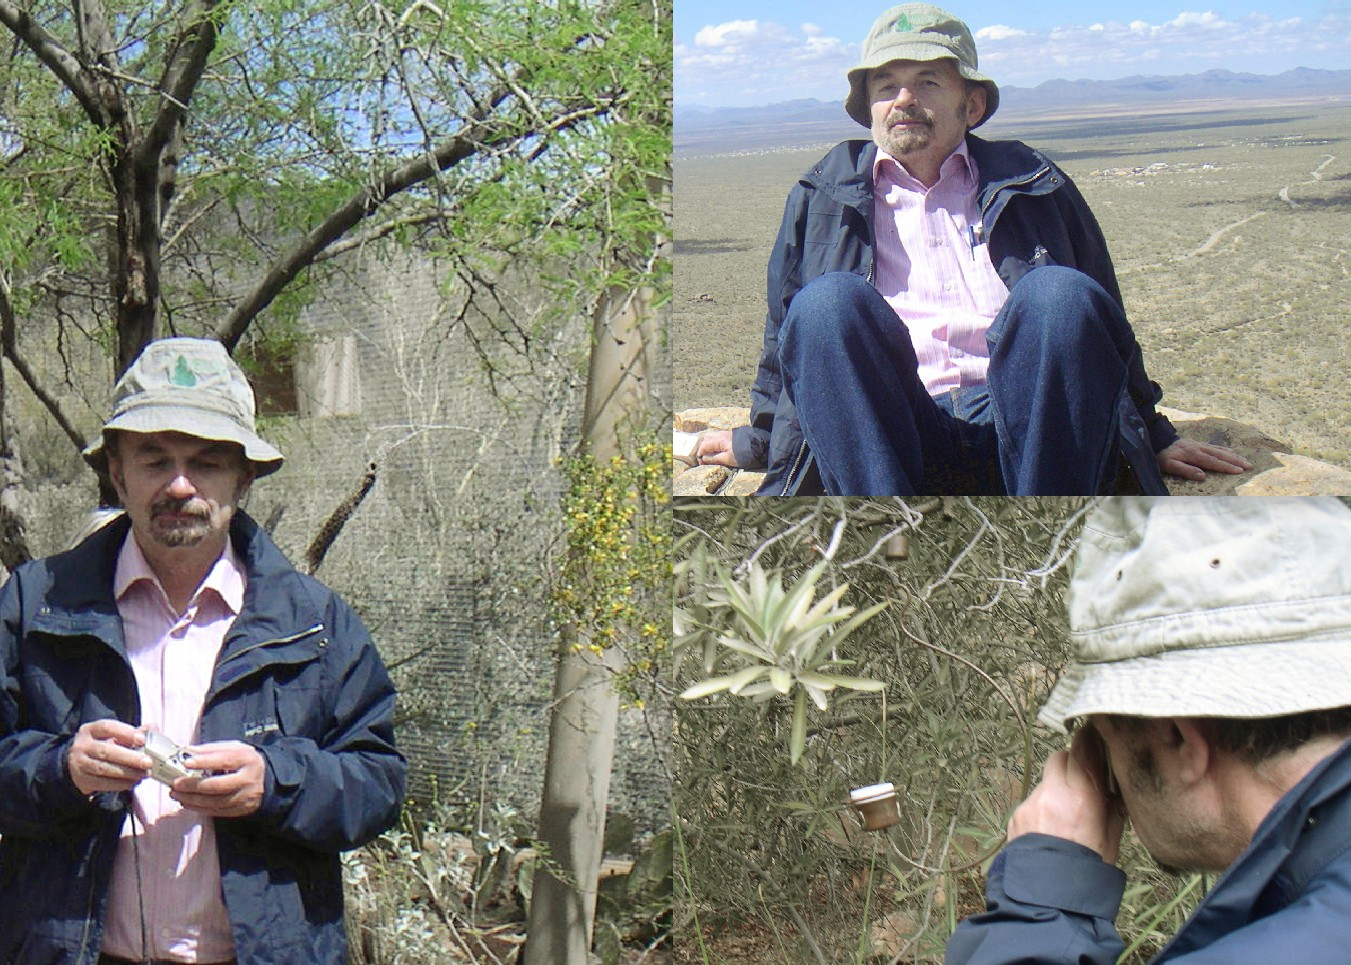
\includegraphics[width=0.95\columnwidth]{07March24HaraldCollageDesertMuseum.jpg}}
\caption{Harald Fritzsch visiting Arizona-Sonora Desert Museum in Spring 2007. Pictures and picture assembly by Johann Rafelski
}
\label{Fig:AZcolloq2007} 
\end{figure}

These meetings offered an opportunity to exchange ideas the  origin of neutrino mass and parameters of  the standard model were close to his heart. Were these parameters really natural constants on cosmological time scale? In Figure\,\ref{Fig:RANP2004} we see Harald's first transparency ``Time Dependence of QCD and Experimental Tests'' made at at the 9th Hadron Physics and 7th Relativistic Aspects of Nuclear Physics (HADRON-RANP 2004): A Joint Meeting on QCD and QGP: Rio de Janeiro, Brazil, March 28-April 3, 2004~\cite{Fritzsch:2004civ}, a meeting we both attended. We see that Harald modified slightly by hand the typed transparency to introduce the meeting specific context in a talk which arose from another publication of the epoch, Ref.\,\cite{Calmet:2001nu}. 

\begin{figure}%[ht]
\centerline{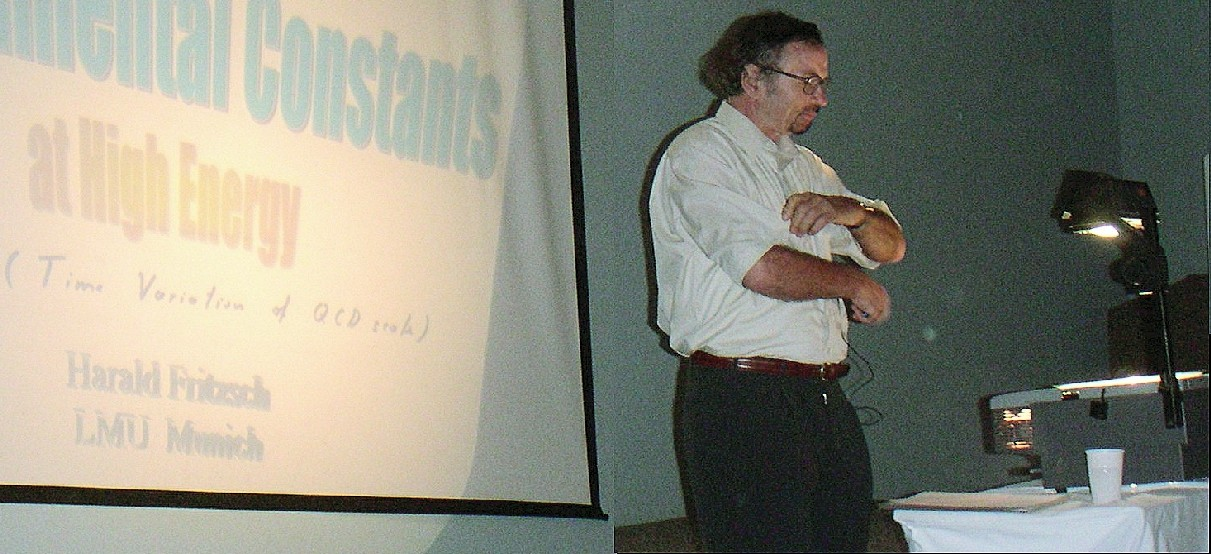
\includegraphics[width=0.95\columnwidth]{04RANPHarald1Ed.jpg}}
\caption{Harald begins his presentation in Rio de Janeiro 2004 about time dependence of QCD, see text for details. Picture by Johann Rafelski
}
\label{Fig:RANP2004} 
\end{figure}
 
%%%%%%%%%%%%%%%%%%%%%%%%%%%%%%%%%%%%


\bibliographystyle{ws-rv-van}
\bibliography{Rafelski_Steinmetz_for_Harald}
%%%%%%%%%%%%%%%%%%%%%%%%%%%%%%%%%%%%
\end{document} 
%%%%%%%%%%%%%%%%%%%%%%%%%%%%%%%%%%%%
